\chapter{Results}%
\label{cha:results}


\section{Toy Example}%
\label{sec:toy_example}

\begin{figure}[htpb] \centering
        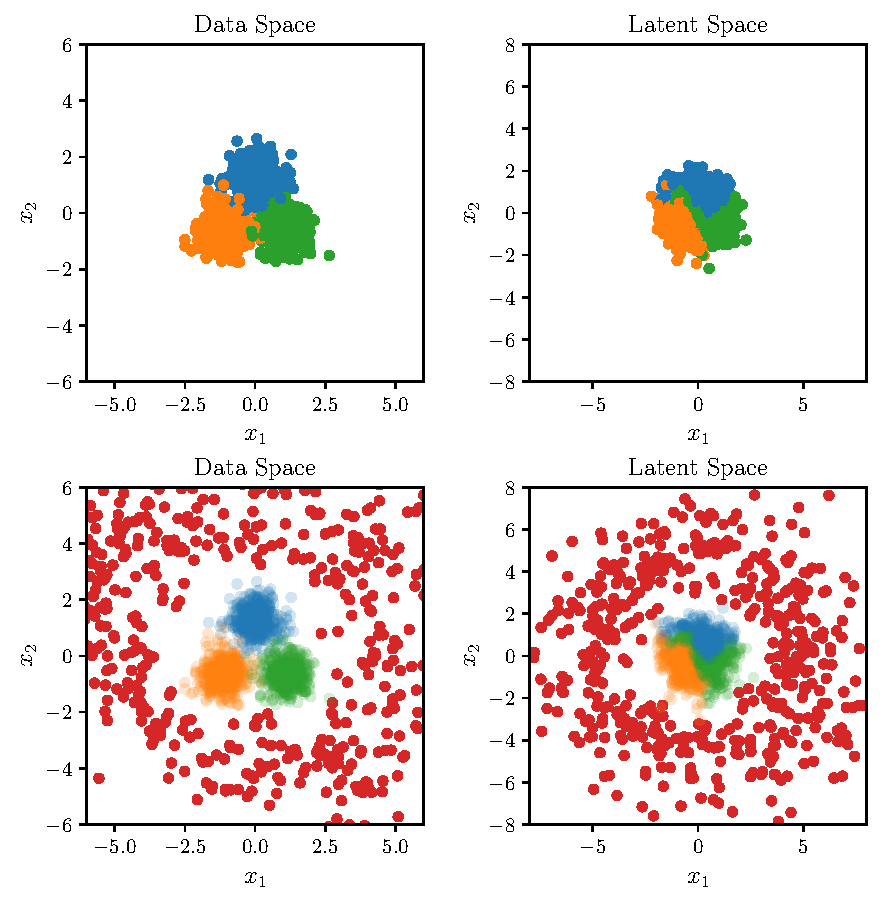
\includegraphics{figures/toy_example/gaussian_mixture/latent_mapping.pdf}
        \caption{\textbf{Top}: Data space and latent space of the Gaussian
        mixture toy dataset. \textbf{Bottom}: The red points are sampled from a
    ring around the latent distribution in latent space and mapped back into
data space with the normalizing flow.}%
	\label{fig:latent_gmm}
\end{figure}

\begin{figure}[htpb]
	\centering
        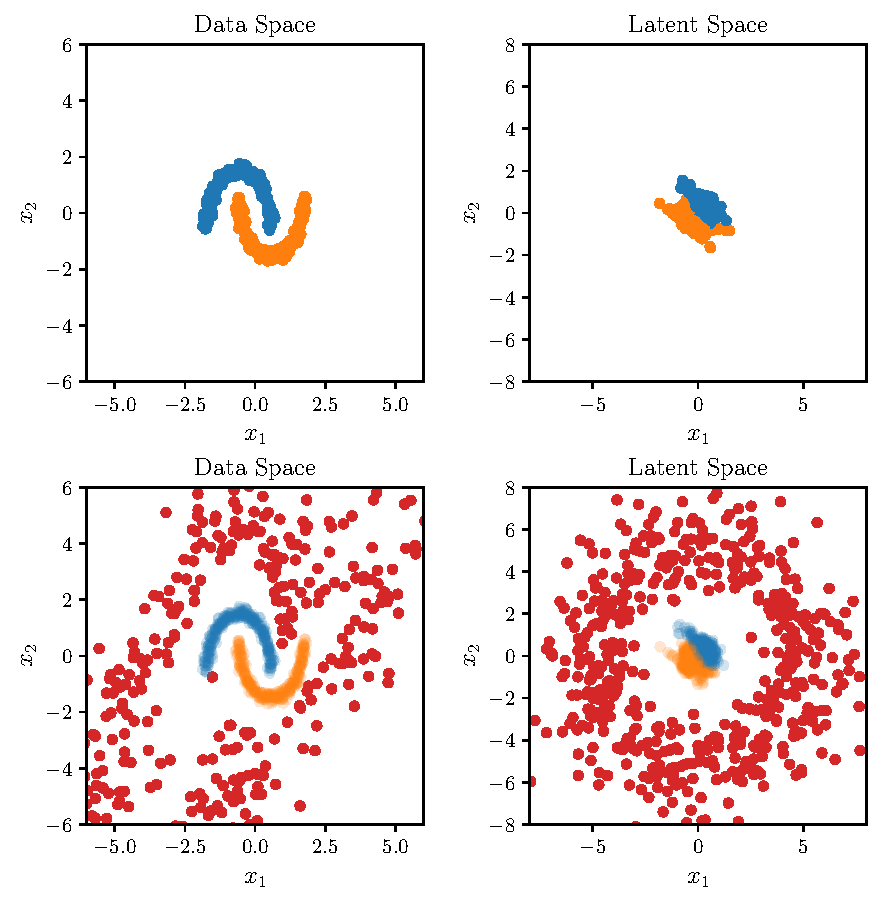
\includegraphics{figures/toy_example/moons/latent_mapping.pdf}
        \caption{\textbf{Top}: Data space and latent space of the Moons
        toy dataset. \textbf{Bottom}: The red points are sampled from a
    ring around the latent distribution in latent space and mapped back into
data space with the normalizing flow.}%
	\label{fig:latent_moons}
\end{figure}

Let us first investigate our methods on some simple toy data. For this we
generate two toy datasets. One dataset consists of three two-dimensional
Gaussian distributions, each being its own class. The other dataset has two
classes shaped like interlocked moons. Both datasets are normalized. On each
dataset we train a simple version of the normalizing flow introduced above. It
consists of three additive coupling blocks, where the coupling
functions are neural networks with five linear layers with rectified linear
units as activation functions. As described in
\autoref{sec:network_architecture}, it is trained to maximize the likelihood of
the training data.
% TODO: why additive

Samples from the Gaussian mixture toy dataset and the learned latent space
is shown in \autoref{fig:latent_gmm}. As we can see
the latent space approximates a standard normal distribution and each class
gets mapped to a region of this distribution.

For the moons toy dataset, samples and the learned latent space are shown in
\autoref{fig:latent_moons}. Again, we observe a reasonable approximation
of a standard normal distribution in the latent space.

% TODO: gumbel params
We can now take a look at the generation of outliers. Since the latent space is
low-dimensional, we use the Gumbel distribution sampling as described in
\autoref{sub:gumbel_distribution}. The sampled ring in
the latent space can be seen in the bottom right of \autoref{fig:latent_gmm} for the
Gaussian mixture dataset and in the bottom right of \autoref{fig:latent_moons} for the
moons dataset. Using the normalizing flow to transform the outlier samples back
to the data space, we get samples that encase the inlier data. For the Gaussian
mixture dataset this can be seen in the bottom left of \autoref{fig:latent_gmm} and
in the bottom left of \autoref{fig:latent_moons} for the moons dataset.

\begin{figure}[htpb]
	\centering
        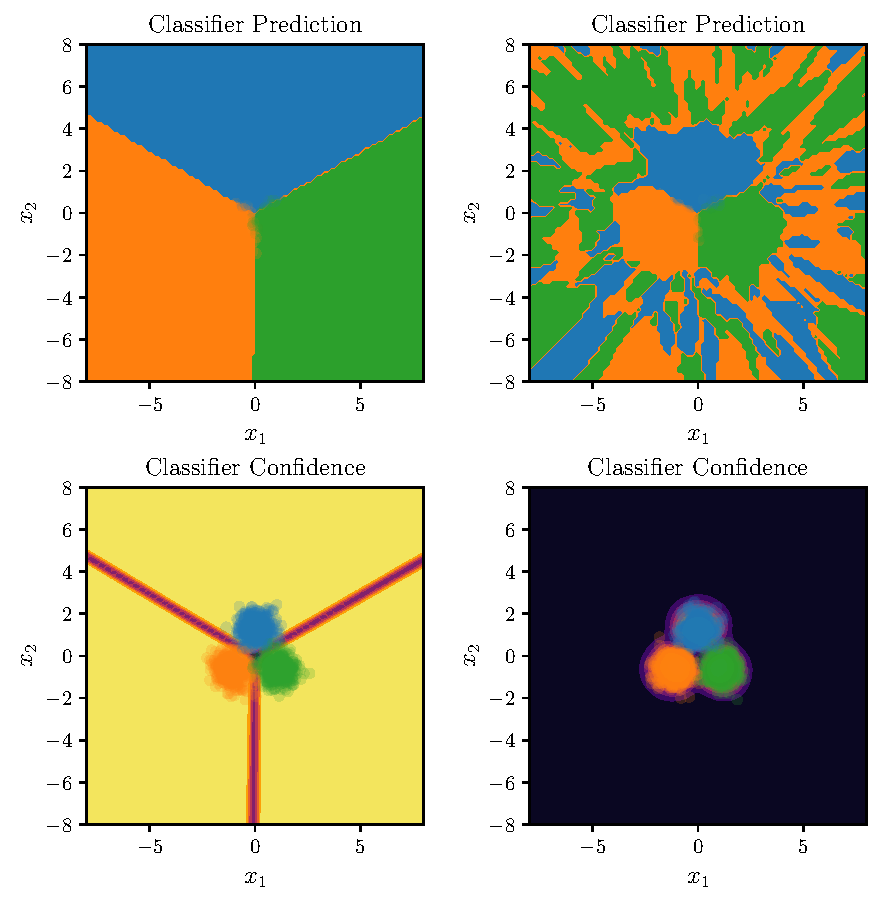
\includegraphics{figures/toy_example/gaussian_mixture/classifier.pdf}
        \caption{\textbf{Left}: Decision regions and confidence of a classifier trained on the
            Gaussian mixture toy dataset. \textbf{Right}: Decision regions and
            confidence of a classifier trained additionally with the
        Kullback-Leibler divergence loss on outliers. In the confidence plots
    higher brightness means higher confidence.}%
	\label{fig:classifier_gmm}
\end{figure}

\begin{figure}[htpb]
	\centering
        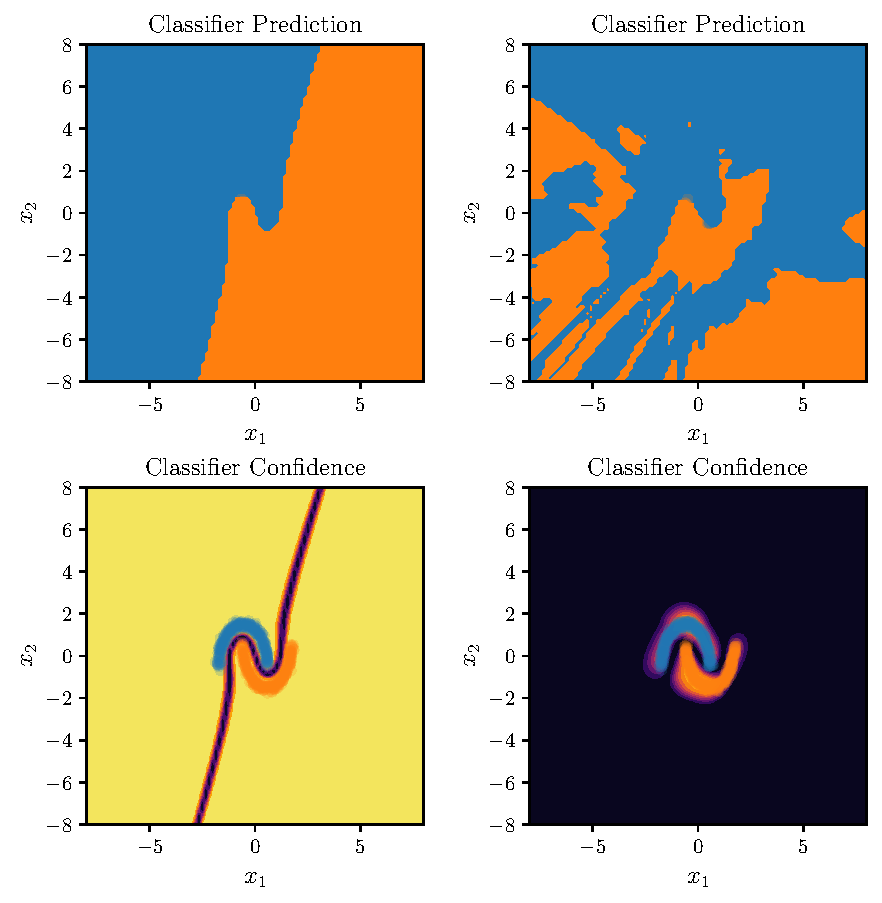
\includegraphics{figures/toy_example/moons/classifier.pdf}
        \caption{\textbf{Left}: Decision regions and confidence of a classifier trained on the
            Moons toy dataset. \textbf{Right}: Decision regions and
            confidence of a classifier trained additionally with the
        Kullback-Leibler divergence loss on outliers. In the confidence plots
    higher brightness means higher confidence.}%
	\label{fig:classifier_moons}
\end{figure}

To show how the generated outliers can be of use, we can train a classifier on
the toy datasets. The classifier is a simple neural network consisting of three
linear layers with rectified linear units as activations. It is trained on the
generated data to minimize the cross-entropy between the ground truth labels
and the predicted labels. This simple setup leads to a classifier that
performs well on both datasets. The decision regions can be seen in the top
right of
\autoref{fig:classifier_gmm} and \autoref{fig:classifier_moons} respectively. To get a
measure of the confidence of the classifier, we can inspect the entropy of the
predicted class distribution. We can see in the bottom left of
\autoref{fig:classifier_gmm} and
\autoref{fig:classifier_moons}, that this classifier has high confidence
everywhere except in a small boundary region between the classes. This is often
undesired as this means outliers remain undetected and receive a oftentimes
wrong class prediction.

This can be mitigated by augmenting the loss of the classifier as described in
\autoref{sec:discriminator_training}. We train the classifier to minimize the
Kullback-Leibler divergence between the predicted class distribution and a
uniform class distribution over the generated outliers. As we can see in the
bottom right of \autoref{fig:classifier_gmm} and \autoref{fig:classifier_moons}
this leads to regions of low confidence all around the data regions while
keeping good decision boundaries in the region of high confidence, shown in the
top left of \autoref{fig:classifier_gmm} and \autoref{fig:classifier_moons}.

\section{Qualitative Comparison}%
\label{sec:qualitative_comparison}

\begin{figure}[htpb]
	\centering
        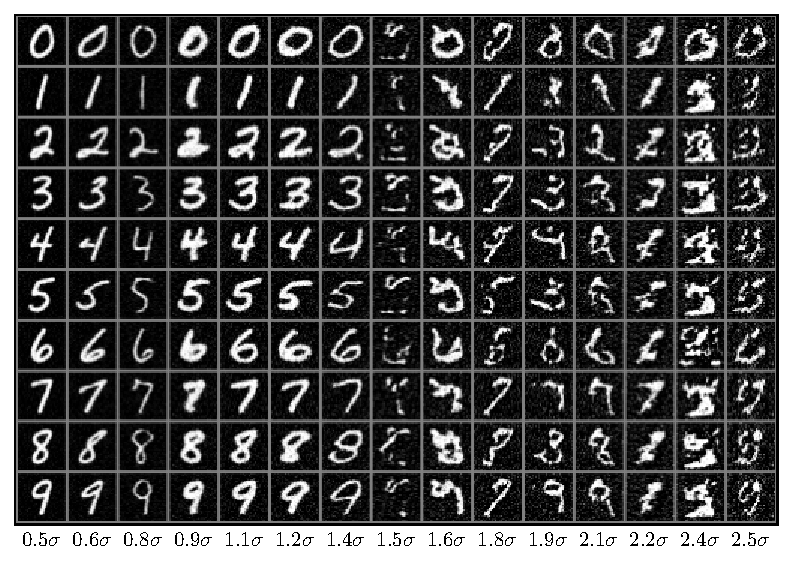
\includegraphics{figures/samples/samples_increasing_distance_EMNIST.pdf}
	\caption{Samples drawn from a multivariate normal distribution and
		mapped back to the data space of the digits dataset. The standard
		deviation in terms of the standard deviation of the data in latent
		space is shown below the images. Each row represents a class, each
		column one sampling variance.}%
	\label{fig:emnist_sample_sigma}
\end{figure}

\begin{figure}[htpb]
	\centering
        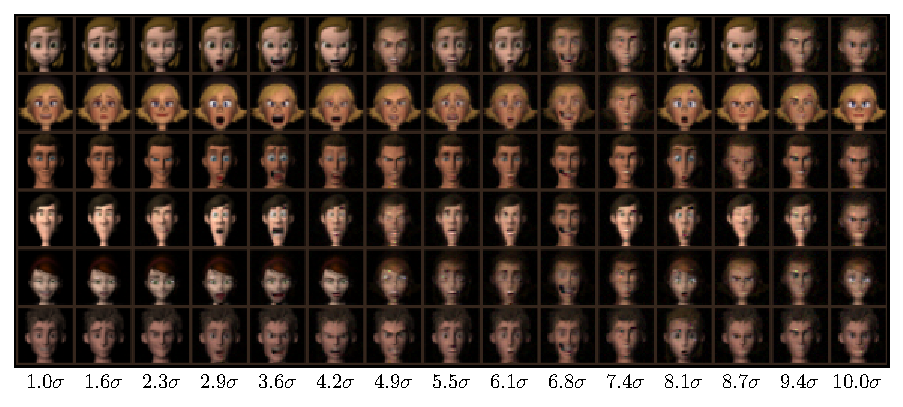
\includegraphics{figures/samples/samples_increasing_distance_FERG_people.pdf}
	\caption{Samples drawn from a multivariate normal distribution and
		mapped back to the data space of the people dataset. The standard
		deviation in terms of the standard deviation of the data in latent
		space is shown below the images. Each row represents a class, each
		column one sampling variance.}%
	\label{fig:ferg_sample_sigma}
\end{figure}

After testing our methods on simple data we can now move on to more complex
data. We now consider the EMNIST dataset as described in
\autoref{sec:datasets}. Again we first train the normalizing flow. In this case
the flow consists of four high-resolution convolutional coupling blocks, four
low-resolution convolutional coupling blocks and two linear coupling blocks.
The flow is trained for 2000 epochs with a learning rate of $10^{-5}$ that gets
reduced by a factor of ten every 600 epochs.

Now we can inspect samples generated from the normalizing flow. Samples are
generated by sampling from a multivariate normal distribution where the
variance has been multiplied by some coefficient as described in
\autoref{sec:extremal_sampling}. The samples with their variance coefficient
are shown in \autoref{fig:emnist_sample_sigma}. Evidently, the images
become increasingly distorted without accumulating much noise, exactly as
expected. Note that the difference in the kind of distortion is that no
particular weight has been placed on structuring the latent space in a
meaningful way and the direction in the latent space is completely random, only
the variance and thereby the radius of the hyperspherical shell has been fixed.
We can also see that images close to the origin are smoother, enabling the
generation of images that could be viewed as prototypical of each class.
Following the discussion in
\autoref{sub:high_dimensional_gaussian_distributions}, we can
easily see how those images are smoother than the majority of the training data
and therefore do not make up the majority of the mass of the distribution.

To consider more complex data, we can repeat this investigation on the people
dataset introduced in \autoref{sec:datasets}. As described above, the dataset
can be ordered by character or by emotion, we choose the character as the class
here. The normalizing flow trained on FERG consists of four high-resolution
convolutional coupling blocks followed by twelve low-resolution convolutional
coupling blocks and twelve linear coupling blocks. It is trained for 1500
epochs with a learning rate of $10^{-4}$ reduced by a factor of ten every 500
epochs. Samples are again generated as in the case of the EMNIST dataset. We
can inspect the samples with their variance coefficients in
\autoref{fig:ferg_sample_sigma}. Apparently one has to sample
much further from the origin in terms of the variance than in the EMNIST case,
suggesting the data is more spread and is approximated worse by a normal
distribution in latent space. We can again see different extreme images that
are unordered, there is again no attention paid to creating meaningful
latent space axes and the sampling direction is random. An interesting effect
to note is, that due to the conditional training different classes can be
noticed to appear as outliers of other classes. We will investigate the
position of classes in the latent space in the next section.
% TODO: investigate gumbel sampling?

\section{Archetypal Analysis}%
\label{sec:archetypal_analysis}

Let us now take a look at sample generation when we additionally add the
archetype mapping to the normalizing flow as described in
\autoref{sec:geometrical_approach}. We first have to consider the choice of the
number of archetypes, for that we follow Keller et
al.~\citep{kellerLearningExtremalRepresentations2020} and train multiple models
with different numbers of archetypes. All models are trained with the
pretrained flow from the previous section. The flow parameters are fixed while
the positions of the archetypes in latent space and the parameters of the
linear mapping layers are trained. We then compute
the mean squared error for the reconstruction of all samples in the training
set. The mean squared error as a function of the number of archetypes for the
EMNIST dataset can be seen in \autoref{fig:emnist_aa_mse}. A reasonable choice
is 14 archetypes, achieving a good reconstruction error while still keeping the
number of archetypes low. For the FERG dataset the mean squared error as a
function of the number of archetypes can be seen in \autoref{fig:ferg_aa_mse},
the ideal choice are seven archetypes. This is notable, because it lines up
with the seven expressions present in the dataset. Indeed,
when showing the sample from each class in the training data that is closest to
the archetypes in \autoref{fig:ferg_aa_closest}, the archetypes can clearly be
identified with the expressions.

\begin{figure}[htpb]
	\centering
	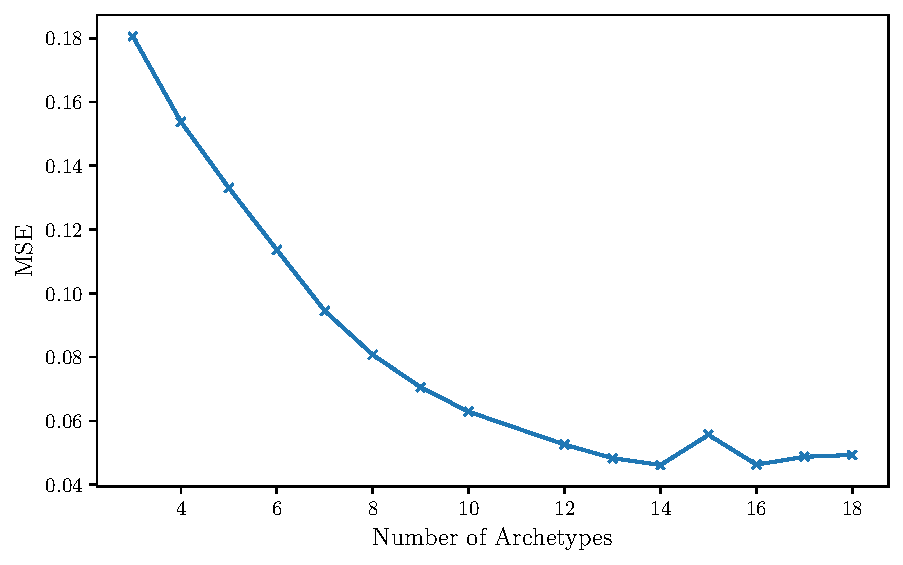
\includegraphics{figures/samples/aa_mse_EMNIST.pdf}
	\caption{Mean squared error when reconstructing the EMNIST training
		dataset as a function of the number of archetypes}%
	\label{fig:emnist_aa_mse}
\end{figure}

\begin{figure}[htpb]
	\centering
	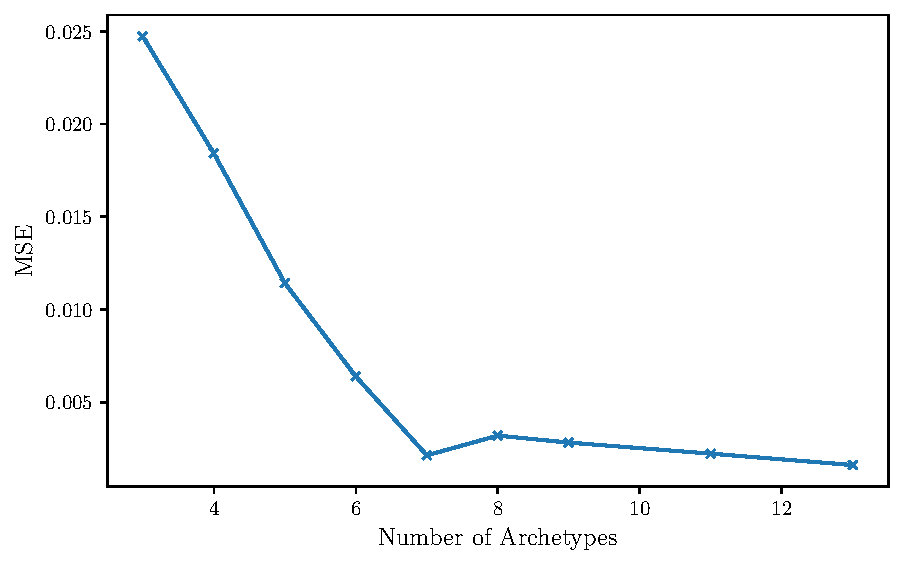
\includegraphics{figures/samples/aa_mse_FERG.pdf}
	\caption{Mean squared error when reconstructing the FERG training
		dataset as a function of the number of archetypes}%
	\label{fig:ferg_aa_mse}
\end{figure}

Note that with an increasing number of archetypes, the
clear interpretability of the individual archetypes is reduced and clearly
distinguishable features become redundant with only subtle differences. This
can be seen when we investigate the images from the training dataset and each
class closest to the archetypes as in \autoref{fig:emnist_aa_closest}.

\begin{figure}[htpb]
	\centering
	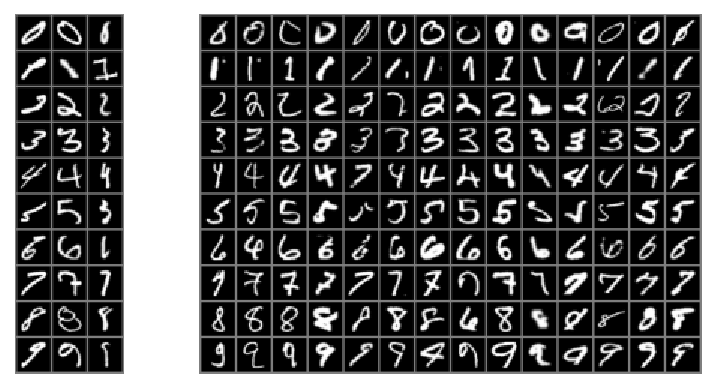
\includegraphics{figures/samples/archetypes_emnist.pdf}
	\caption{The images from the EMNIST dataset closest to each of the
		archetypes of the model with three and the model with 14 archetypes
		respectively.}%
	\label{fig:emnist_aa_closest}
\end{figure}

\begin{figure}[htpb]
	\centering
	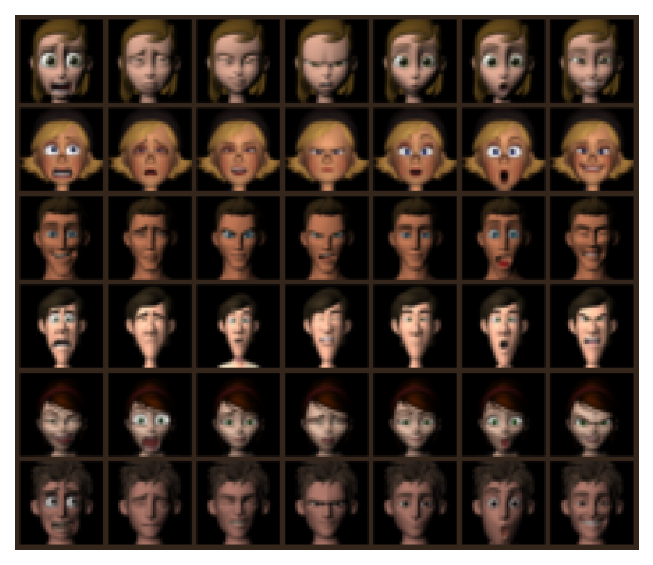
\includegraphics{figures/samples/archetypes_ferg_7.pdf}
	\caption{The images from the FERG dataset closest to each of the
		archetypes of the model.}%
	\label{fig:ferg_aa_closest}
\end{figure}

\autoref{fig:aa_emnist} depicts samples generated by sampling from a
Dirichlet distribution and mapping those samples back into the data space of
the EMNIST dataset. To identify extreme samples, or outliers, we can
change the shape parameters of the Dirichlet distribution to draw samples close
to one of the archetypes. \autoref{fig:aa_emnist_corners} shows such samples as
well as how the images are distorted in specific ways
related to the archetype. This could allow, for example, to investigate what
extreme points in the data may look like and obtain an intuition for outliers
that could act as adversarial data points.
The same experiment can be done with the model trained on the FERG dataset.

Turning to \autoref{fig:aa_ferg} and \autoref{fig:aa_ferg_corners}, we
are again able to generate in-distribution samples and also extreme samples,
where the distorted features are again controlled by the archetypes via the
shape parameters of the Dirichlet distribution. Notably, extreme samples
generated are also more distorted then the samples closest to the archetypes
from the dataset shown in \autoref{fig:emnist_aa_closest} and
\autoref{fig:ferg_aa_closest}.

\begin{figure}[htpb]
	\centering
	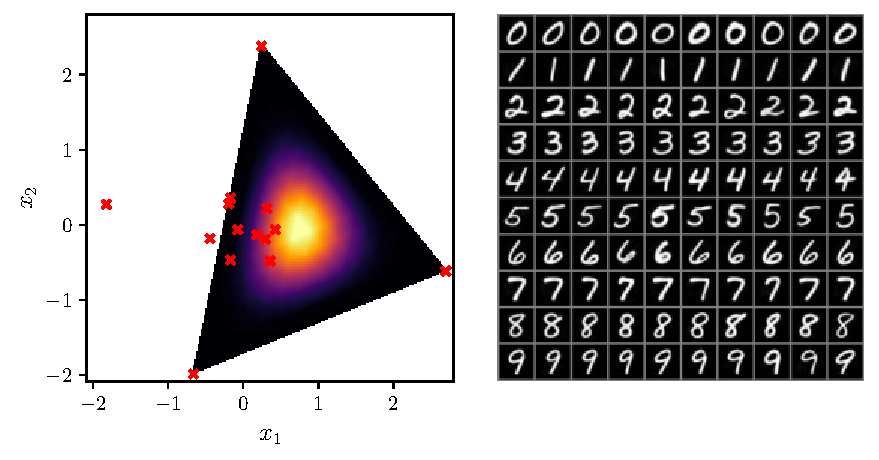
\includegraphics[width=1\linewidth]{figures/samples/aa_emnist.pdf}
	\caption{Samples drawn from a dirichlet distribution and mapped back to
		the data space of the EMNIST dataset. On the \textbf{left} hand side the
		probability density function of the latent samling distribution is
		shown, on the \textbf{right} the resulting samples are shown. Each row
		corresponds to one class.}%
	\label{fig:aa_emnist}
\end{figure}

\begin{figure}[htpb]
	\centering
	\begin{subfigure}[htpb]{\textwidth}
		\centering
		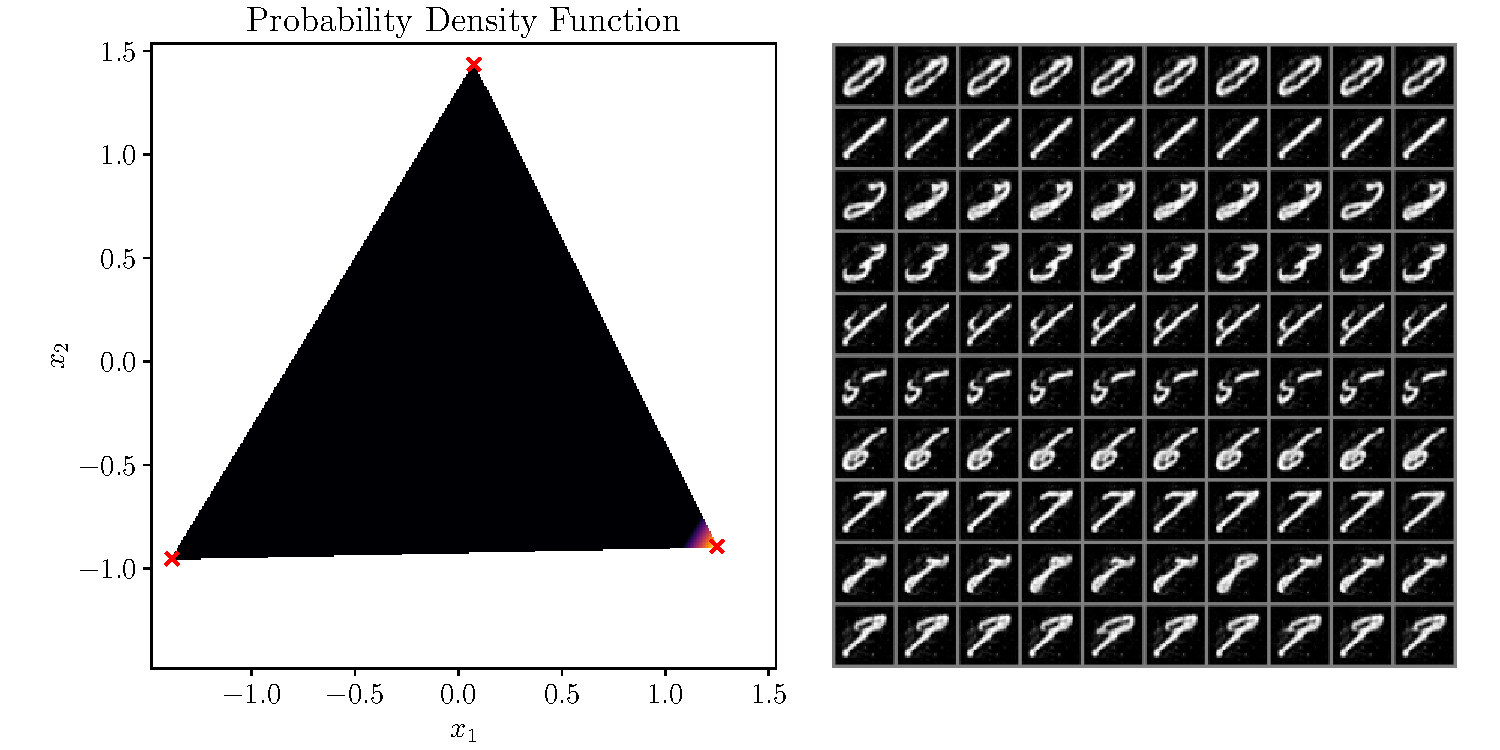
\includegraphics[width=1\linewidth]{figures/samples/aa_emnist1.pdf}
	\end{subfigure}

	\begin{subfigure}[htpb]{\textwidth}
		\centering
		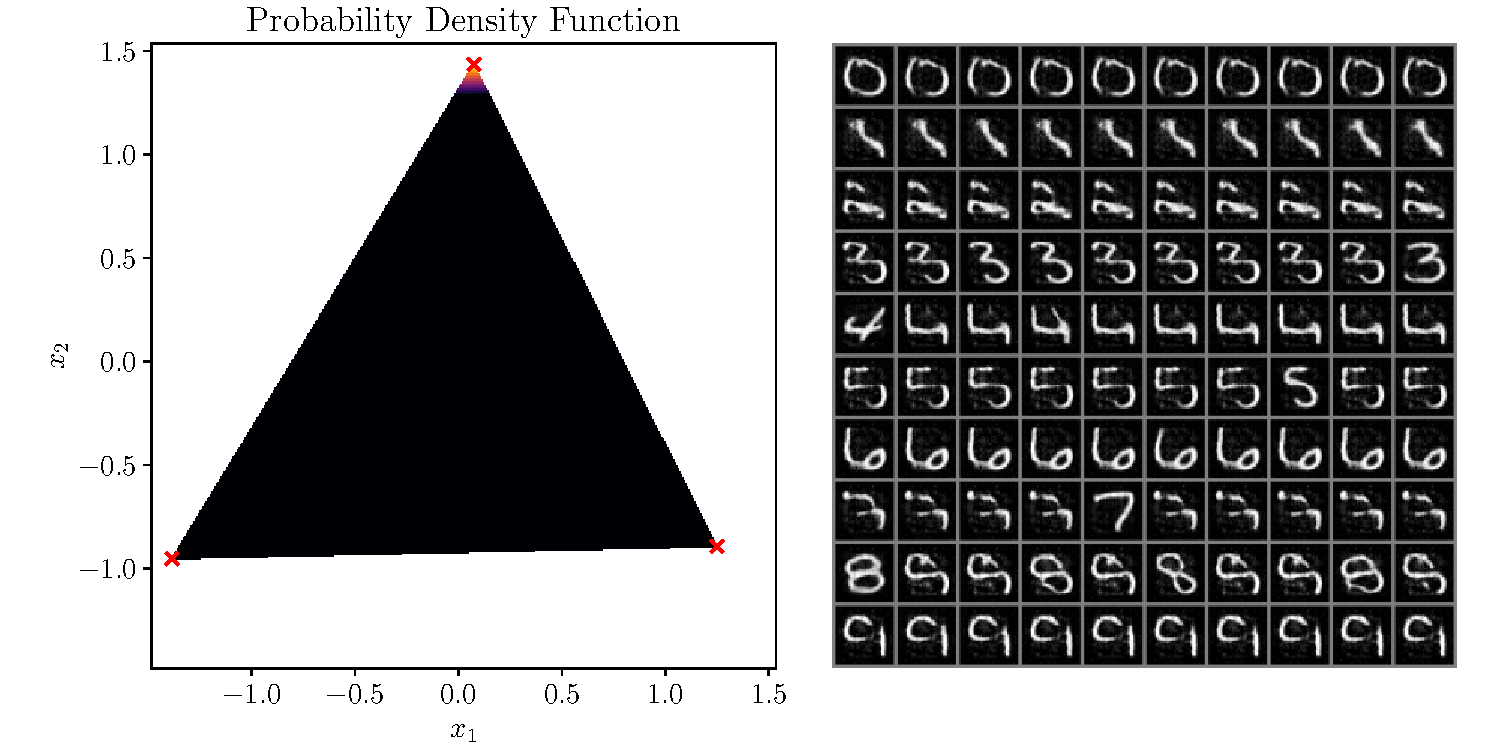
\includegraphics[width=1\linewidth]{figures/samples/aa_emnist2.pdf}
	\end{subfigure}

	\begin{subfigure}[htpb]{\textwidth}
		\centering
		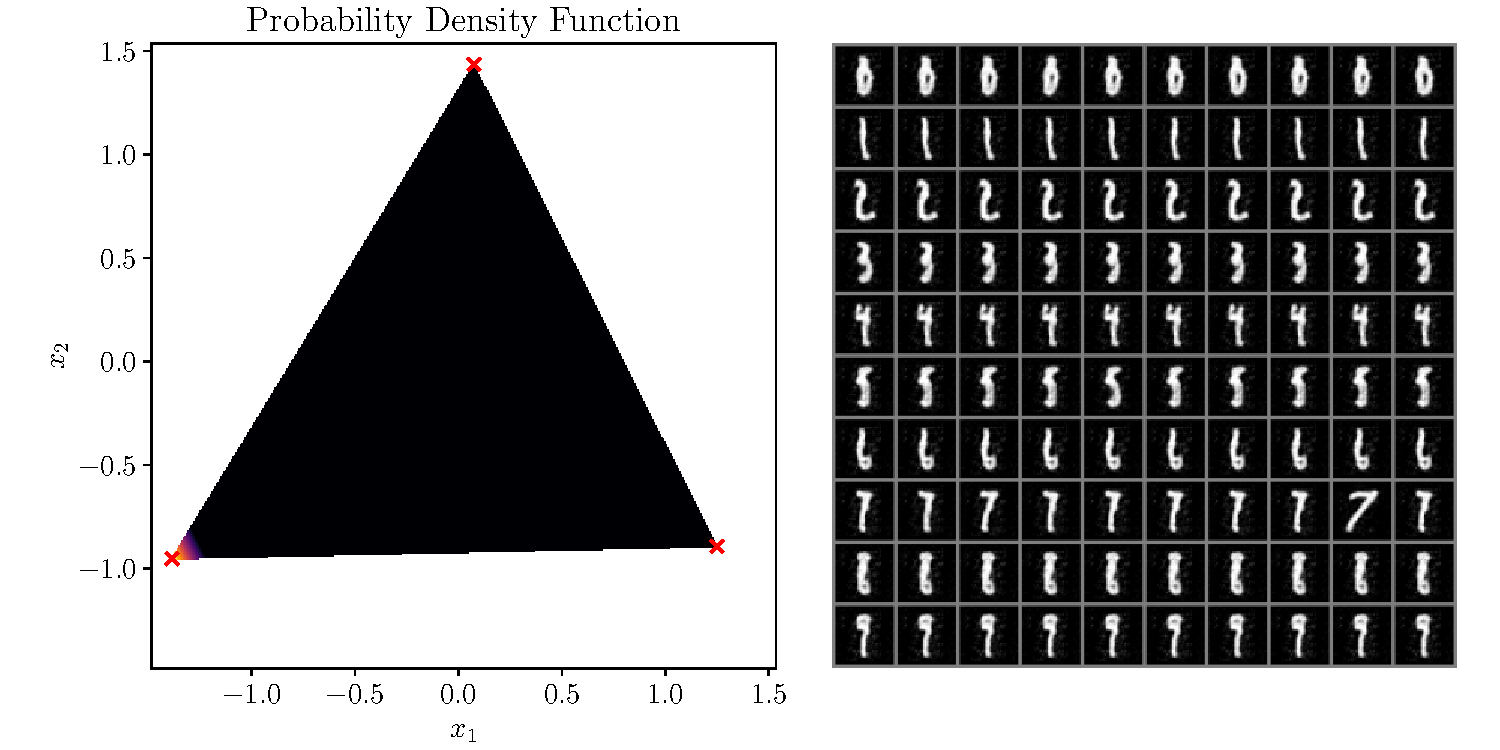
\includegraphics[width=1\linewidth]{figures/samples/aa_emnist3.pdf}
	\end{subfigure}
	\caption{Samples drawn from a dirichlet distribution and mapped back to
		the data space of the EMNIST dataset. \textbf{Top},
                \textbf{mid} and \textbf{bottom} show sampling
		close to one archetype each.}%
	\label{fig:aa_emnist_corners}
\end{figure}

\begin{figure}[htpb]
	\centering
	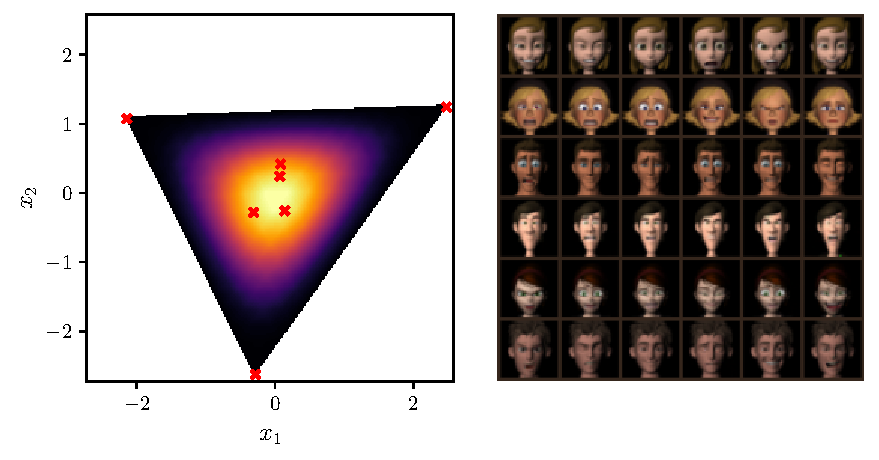
\includegraphics[width=1\linewidth]{figures/samples/aa_ferg.pdf}
	\caption{Samples drawn from a dirichlet distribution and mapped back to
		the data space of the FERG dataset. On the \textbf{left} hand side a
		projection of the probability density function of the latent
		sampling distribution is shown, on the \textbf{right} the resulting samples
		are shown. Each row corresponds to one class.}%
	\label{fig:aa_ferg}
\end{figure}

\begin{figure}[htpb]
	\centering
	\begin{subfigure}[htpb]{\textwidth}
		\centering
		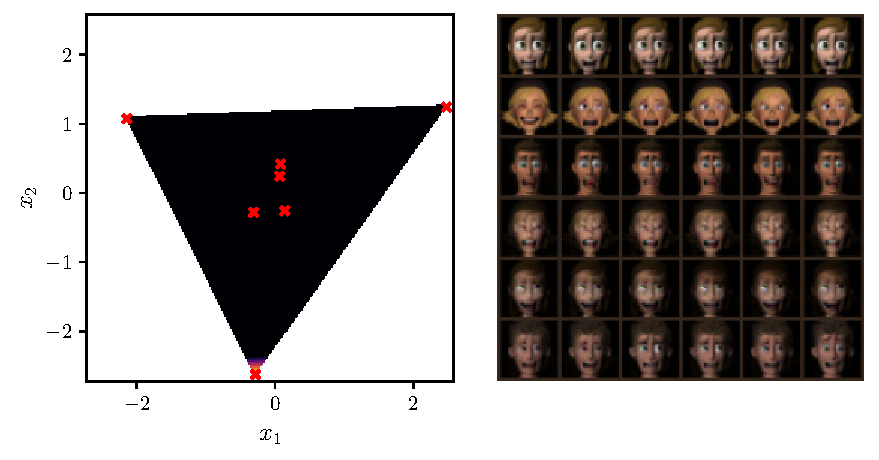
\includegraphics[width=1\linewidth]{figures/samples/aa_ferg1.pdf}
	\end{subfigure}

	\begin{subfigure}[htpb]{\textwidth}
		\centering
		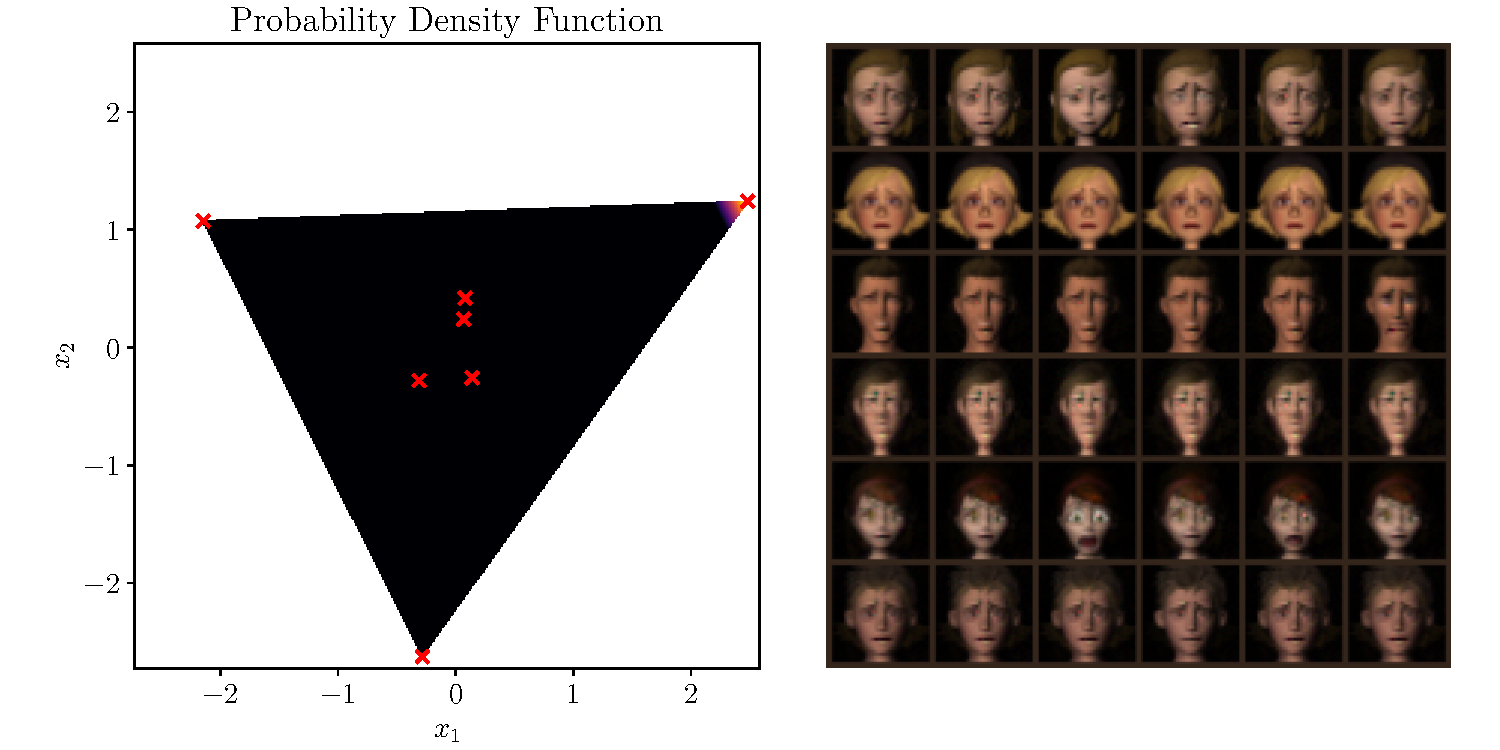
\includegraphics[width=1\linewidth]{figures/samples/aa_ferg2.pdf}
	\end{subfigure}

	\begin{subfigure}[htpb]{\textwidth}
		\centering
		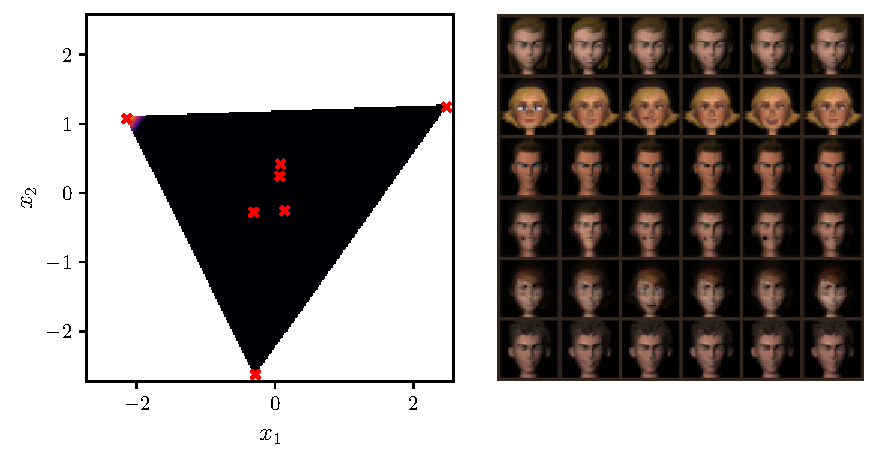
\includegraphics[width=1\linewidth]{figures/samples/aa_ferg3.pdf}
	\end{subfigure}

	\caption{Samples drawn from a dirichlet distribution and mapped back to
		the data space of the FERG dataset. \textbf{Top}, \textbf{mid}
                and \textbf{bottom} show
		sampling close to one archetype each.}%
	\label{fig:aa_ferg_corners}
\end{figure}

\subsection{Nullspace Sampling}%
\label{sub:nullspace_sampling}

For the EMNIST dataset, the number of archetypes needed to achieve a low
reconstruction error is surprisingly high. Another way to improve
reconstructions, and thereby the quality of generated samples, is augmenting the
samples with samples from the nullspace of the mapping to archetype space. This
works especially well when using no bias in the mapping. A model with three
archetypes and no bias thereby achieves a mean squared reconstruction error of
$0.022$ on EMNIST, lower than any of the models achieved without augmentation
(see \autoref{fig:emnist_aa_mse}). A model with bias in the mapping can still
achieve a mean squared error on EMNIST of $0.068$, which is an improvement
equivalent to tripeling the number of archetypes. In \autoref{fig:aa_nullspace}
we can see how this affects samples from the center of the simplex and each of
the corners.
\begin{figure}[htpb]
	\centering
		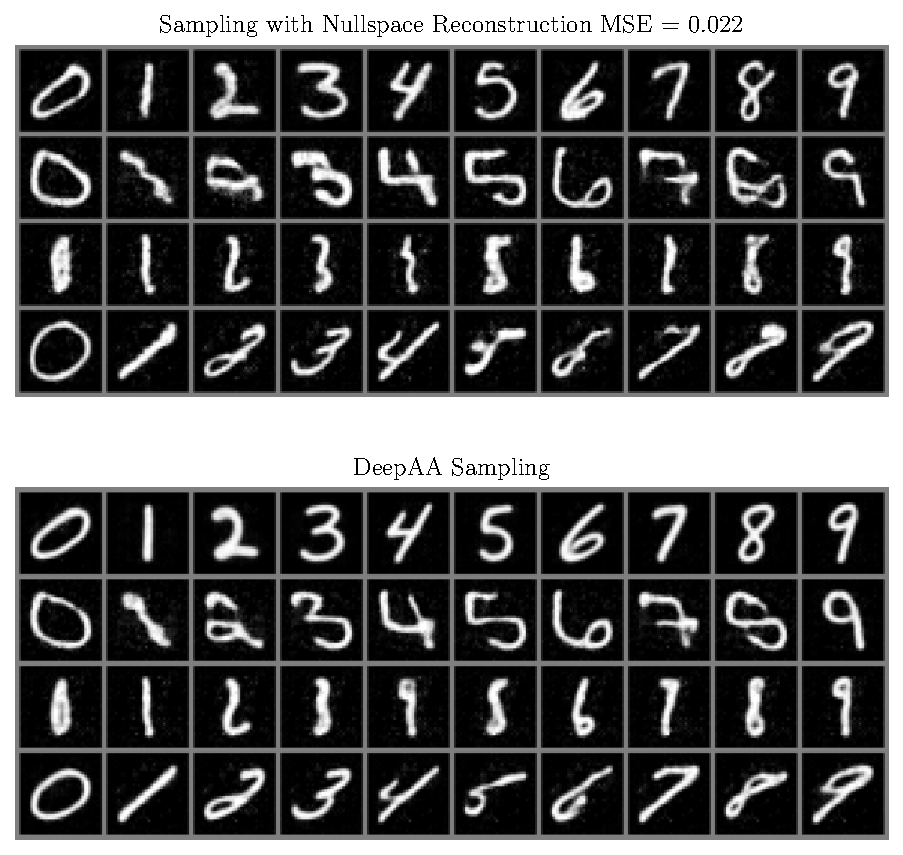
\includegraphics{figures/samples/aa_nullspace.pdf}
	\caption{Samples from the center of the Dirichlet distribution and each
		of the corners. Each column is one class. \textbf{Top}: Model without bias in
		the mapping to archetype space. \textbf{Bottom}: Model with bias in the mapping to
		archetype space.}%
	\label{fig:aa_nullspace}
\end{figure}
\begin{figure}[htpb]
	\centering
        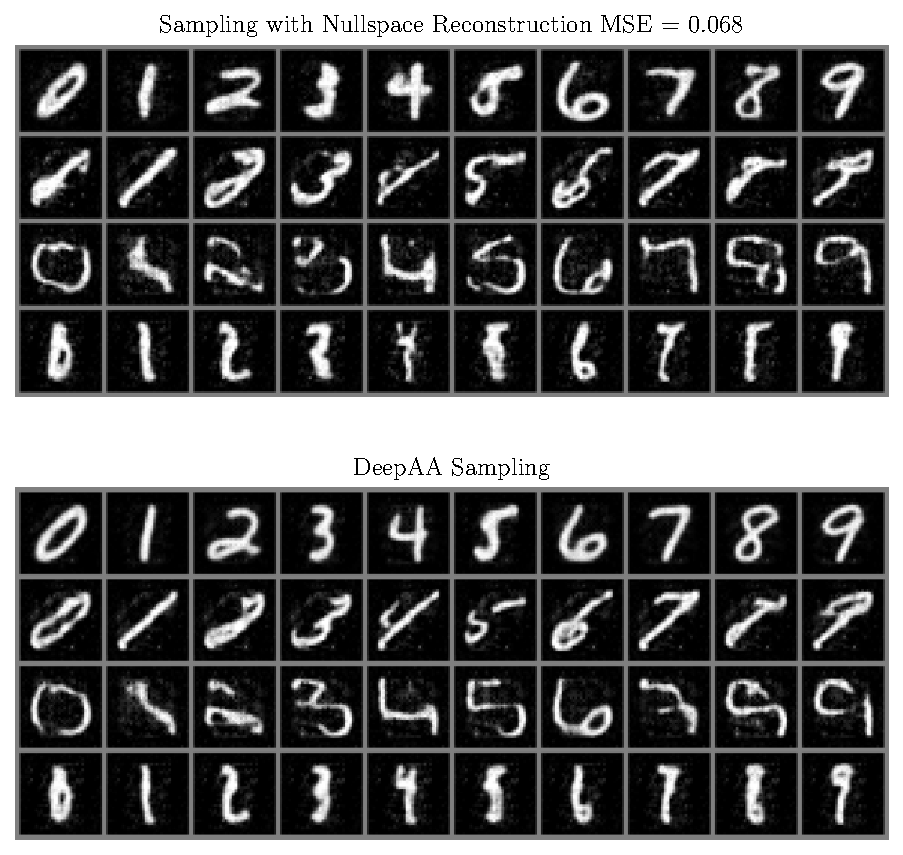
\includegraphics{figures/samples/aa_nullspace_bias_y.pdf}
        \caption{Samples from the center of the Dirichlet distribution and each
        of the corners. Each column is one class. \textbf{Top}: Model without bias in
        the mapping to archetype space. \textbf{Bottom}: Model with bias in the mapping to
        archetype space.}%
        \label{fig:aa_nullspace_bias}
\end{figure}

\section{Analysis of the Latent Space}%
\label{sec:analysis_of_the_latent_space}

After investigating the models qualitatively, we will now look more closely
into the latent space and how different samples and classes relate to each
other. Our investigation begins with EMNIST.

To check our intuition, that classes that are similar to each other visually
should be placed close to each other in latent space we can check cluster
distances between classes. For that we compute the latent vectors of the data
in question conditioned on each of the classes in EMNIST. To ease computation
and visualization we perform a linear discriminant analysis on each of the class
pairs and project the data on the first two components of the linear
discriminant analysis. Next, we compute the mean euclidean distance of 1000
sample pairs from the two classes. The result is shown as a colored matrix in
\autoref{fig:emnist_distance_matrix} for a comparison of EMNIST to itself and
in \autoref{fig:emnist_distance_matrix_letters} for a comparison to the letters
dataset. As expected, classes that are visually similar are close together:
Consider, for example, how the class \texttt{6} is close to class \texttt{0}
when the network is conditioned on class \texttt{0}, but also more unexpected
relations are revealed, such as class \texttt{9} being
close to class \texttt{4} when conditioned on \texttt{4} and class \texttt{2}
being close to class \texttt{8} when
conditioned on \texttt{8}. Also notable is the asymmetry of the matrix. This is due to
the fact that the class conditioning makes the flow maximize the likelihood of
samples of the class matching the condition, while the combination of a class
condition with a foreign class sample is unseen during training and therefore
does not influence the latent space layout.

Our intuition on the placement of visually similar classes is also confirmed
when looking at samples from a dataset of outliers, in this case the letters
dataset. Notably, the class \texttt{O} from the letters dataset is close to the
class \texttt{0} when conditioned on \texttt{0}, as one would expect.
Similarly, \texttt{i} and \texttt{1}, and \texttt{p} and \texttt{8} or
\texttt{9} are close.

\begin{figure}[htpb]
	\centering
	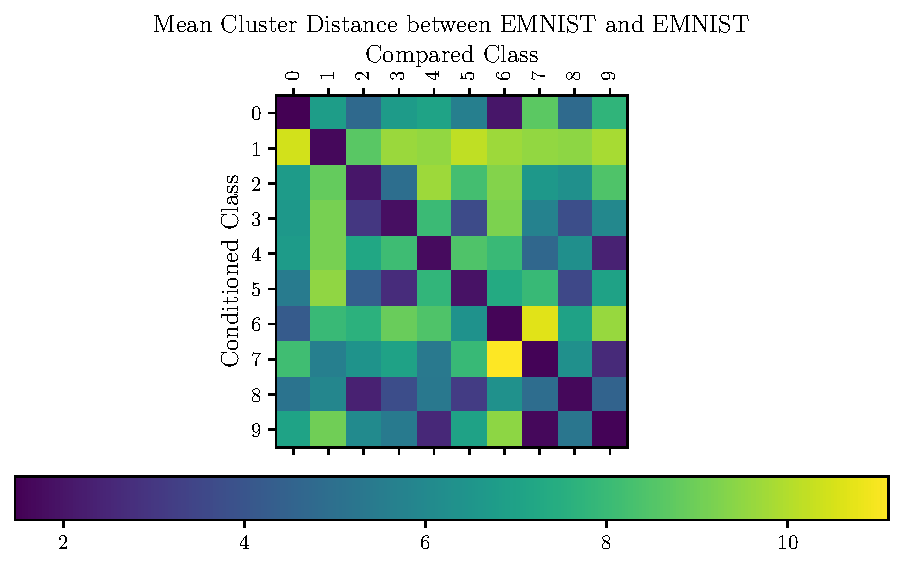
\includegraphics{figures/samples/emnist_distance_matrix_EMNIST_lda.pdf}
	\caption{Mean distance in LDA projection space between samples from the
		conditioning class (y axis) and a test class (x axis). Classes and
		samples are from the EMNIST dataset. Darker means closer
		together.}%
	\label{fig:emnist_distance_matrix}
\end{figure}

\begin{figure}[htpb]
	\centering
	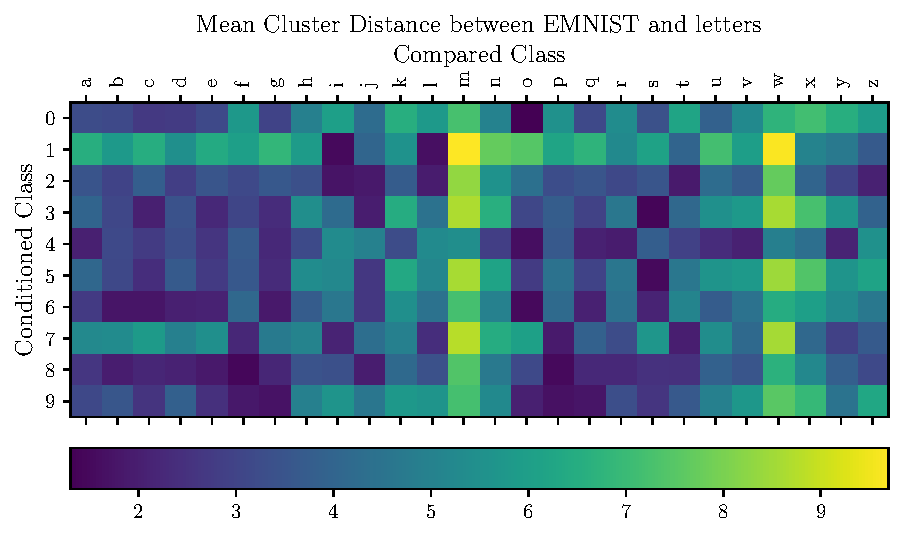
\includegraphics{figures/samples/emnist_distance_matrix_letters_lda.pdf}
	\caption{Mean distance in LDA projection space between samples from the
		conditioning class (y axis) and a test class (x axis). Samples
		from the conditioning class are from the EMNIST dataset, test
		samples are from the letters dataset. Darker means closer
		together.}%
	\label{fig:emnist_distance_matrix_letters}
\end{figure}

For the FERG dataset relations between classes are less intuitive than for the
EMNIST dataset. Still, we can look at the distances of samples from test
classes to a conditioning class in \autoref{fig:ferg_distance_matrix}. Most
notable here is, that although all images are somewhat similar since they are
computer generated, the classes \texttt{jules} and \texttt{ray} are clustered
close to all other classes.
In contrast to EMNIST we do not have a dataset of close outliers for the FERG
dataset. To still make some measurements with models trained on the FERG
dataset we use CIFAR10 as a source of outliers. The matrix of pairwise
distances can be seen in \autoref{fig:ferg_distance_matrix_cifar}. It is again
interesting to see, that different classes are closer or further away not to
specific other classes but to the dataset as a whole.

\begin{figure}[htpb]
	\centering
	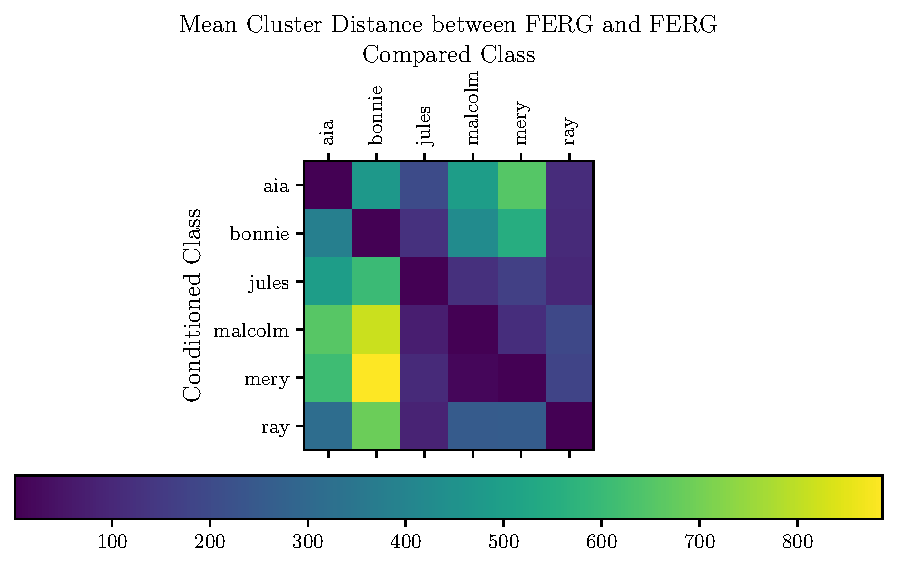
\includegraphics{figures/samples/ferg_distance_matrix_ferg_lda.pdf}
	\caption{Mean distance in LDA projection space between samples from the
		conditioning class (y axis) and a test class (x axis). Samples
		are from the FERG dataset. Darker means closer together.}%
	\label{fig:ferg_distance_matrix}
\end{figure}

\begin{figure}[htpb]
	\centering
	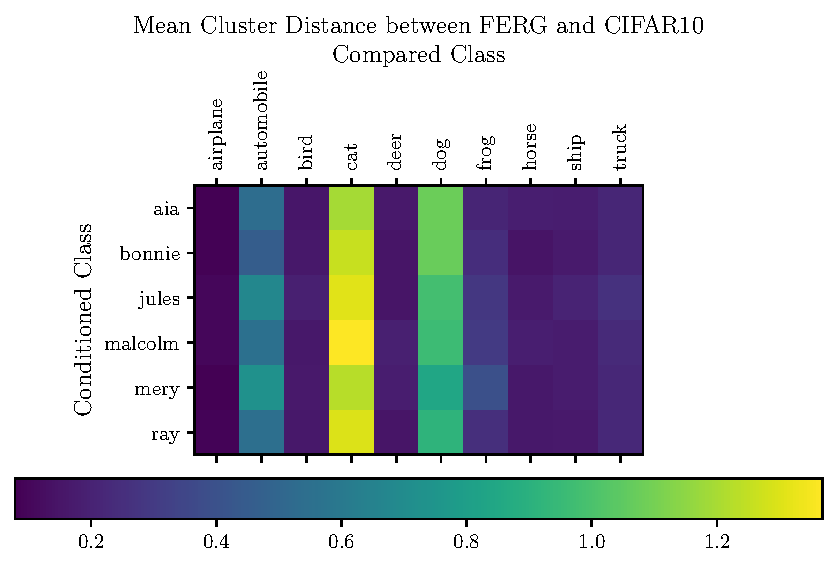
\includegraphics{figures/samples/ferg_distance_matrix_cifar_lda.pdf}
	\caption{Mean distance in LDA projection space between samples from the
		conditioning class (y axis) and a test class (x axis). Samples
		from the conditioning class are from the FERG dataset, test
		samples are from the CIFAR10 dataset. Darker means closer
		together.}%
	\label{fig:ferg_distance_matrix_cifar}
\end{figure}

Since our method of sampling outliers relies on sampling on a shell around the
inlier distribution as a whole and not the position of specific types of
outliers, we will now look at the distribution of the lengths of latent
vectors. For EMNIST, the distribution of latent vector lengths of inlier data
and from the outlier datasets letters, FashionMNIST and KMNIST are shown in
\autoref{fig:emnist_radius_hist}. We can see that the letters dataset is close
to the EMNIST dataset and even has some overlap, while the other two datasets
are further away. To show where the overlap might come from we again look at
the distribution of latent vector lengths in
\autoref{fig:emnist_radius_hist_xo} but constrain the data to the classes
\texttt{o} and \texttt{x}. Following our intuition the letters class \texttt{o}
has a similar latent vector length distribution as the EMNIST class \texttt{0}
while \texttt{x} is more clearly an outlier class by our measure.

\begin{figure}[htpb]
	\centering
	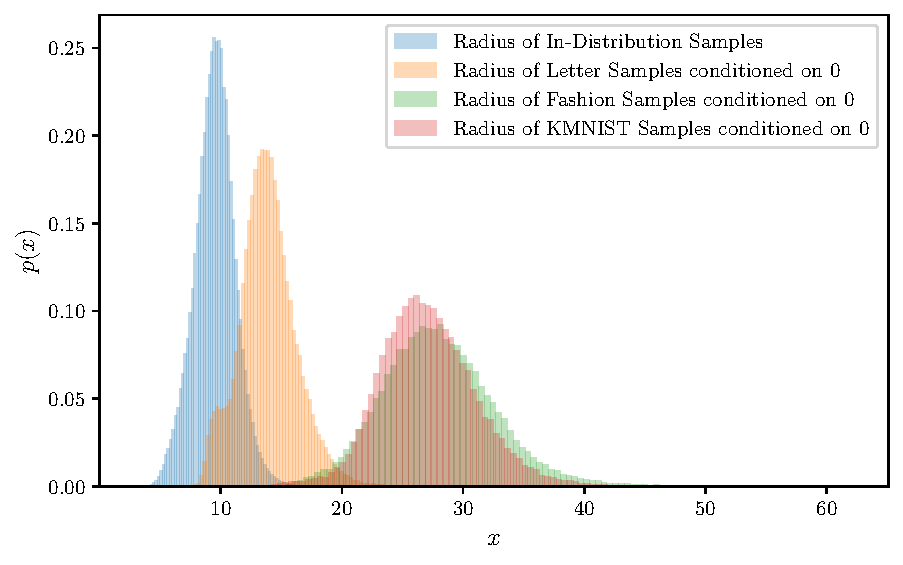
\includegraphics{figures/samples/emnist_radius_hist.pdf}
	\caption{Distribution of the length of latent space vectors for EMNIST
		and its outlier datasets.}%
	\label{fig:emnist_radius_hist}
\end{figure}

\begin{figure}[htpb]
	\centering
	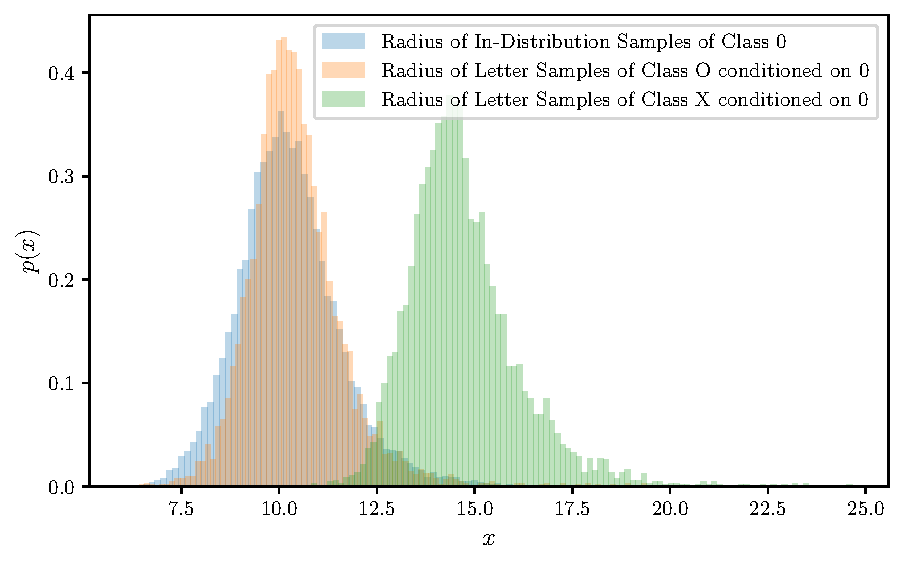
\includegraphics{figures/samples/emnist_radius_hist_xo.pdf}
	\caption{Distribution of the length of latent space vectors for
		\texttt{0} compared with \texttt{o} and \texttt{x}.}%
	\label{fig:emnist_radius_hist_xo}
\end{figure}


\section{Discriminator Performance}%
\label{sec:discriminator_performance}

To show a potential application of the outlier generation we train
discriminator and classification networks on using the models we investigated
above. The architecture and training is described in
\autoref{sec:discriminator_training}. As the source of outliers we use
different settings for our normalizing flow network, sampling with various
standard deviations, sampling from a Gumbel distribution and sampling from a
Dirichlet distribution with various shape parameters. We compare this to using
the letters and fashion datasets directly as outliers when taking the digits
dataset as inliers. Similarly, we compare our networks to using CIFAR10 as a
source of outliers when using the people dataset as inliers. To compare the
results we plot the precision-recall (PR) and receiver operating characteristic
(ROC) curves for each of the models and compute the average precision and area
under the ROC curve.

Taking the digits dataset as the source of inliers we train the discriminator
and classification models for ten epochs. The curves as described above can be
seen in \autoref{fig:emnist_stat_disc} for the discriminators and in
\autoref{fig:emnist_stat_class} for the classifiers. For the normalizing flow
(INN), $p$ denotes the coefficient with which the standard deviation in latent
space is multiplied, or a multiplicative factor controlling the mean and
standard deviation of the Gumbel distribution. The models with archetypal
analysis (DeepAA) receive samples from a Dirichlet distribution where all shape
parameters are equal $c_1 = \dots = c_k = p$. Especially interesting is seeing
the performance when the letters dataset is used, since this dataset is the
most similar to the digits dataset and thereby the most challenging to
distinguish. Both the normalizing flow and the archetype model achieve good
performance on this task that is close to the discriminator trained directly on
the letters dataset. It is also interesting to see, that performance greatly
depends on the parameters that control the outlier distribution in latent
space, where the performance suffers when the distribution is too close to the
inliers as well as when it is too far away. With the classifier we can also
note, that classification performance is not impacted by the addition of the
outlier loss. We observe similar performance when using the people dataset as
inliers, although this measurement is not as meaningful as the previous one,
since there is no good source of outliers to compare against. This is most
notable when looking at the classifier performance in \autoref{tab:ferg_class},
where all classifiers perform extremely well against the CIFAR10 dataset,
except the classifier with no outlier loss at all.

\begin{figure}[htpb]
    \centering
    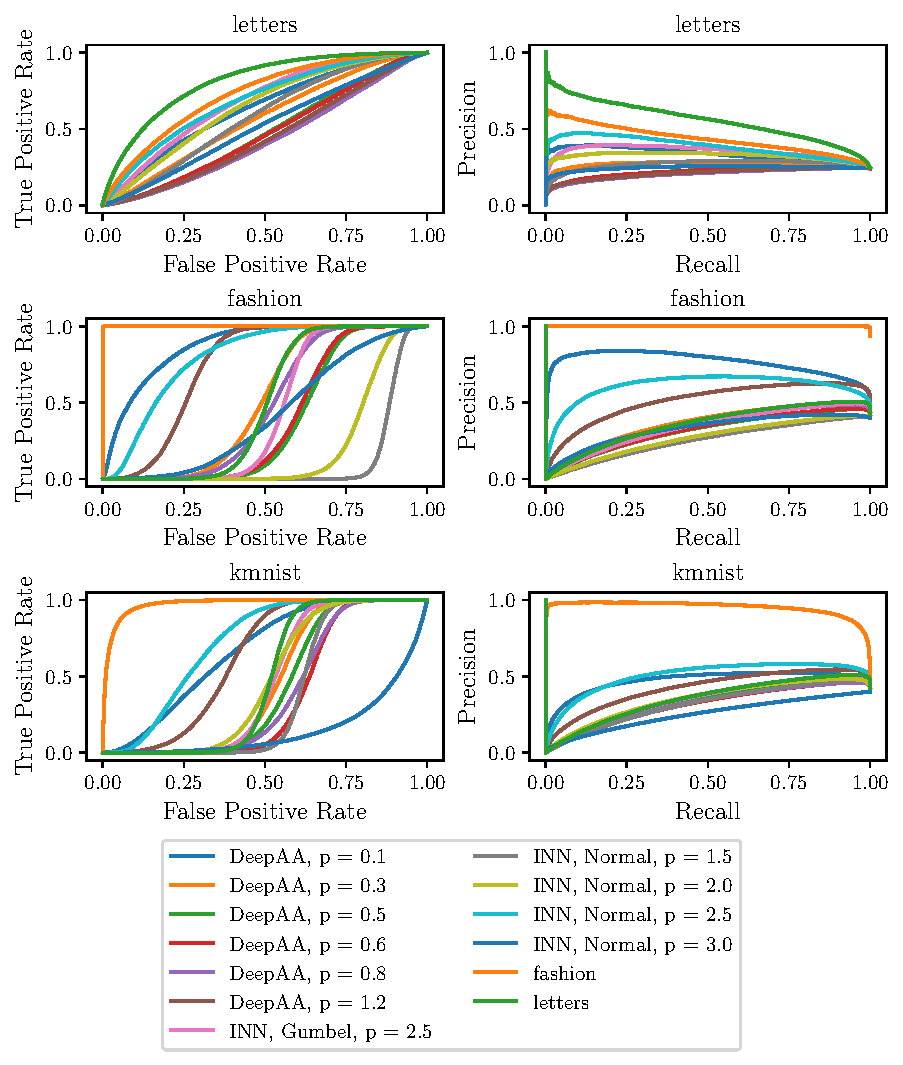
\includegraphics{figures/samples/emnist_disc_curve.pdf}
    \caption{ROC curves (\textbf{left}) and precision-recall curve (\textbf{right}) for
    discriminators trained on different sources of outliers tested on different
    sources of outliers.}%
    \label{fig:emnist_stat_disc}
\end{figure}

\begin{figure}[htpb]
    \centering
    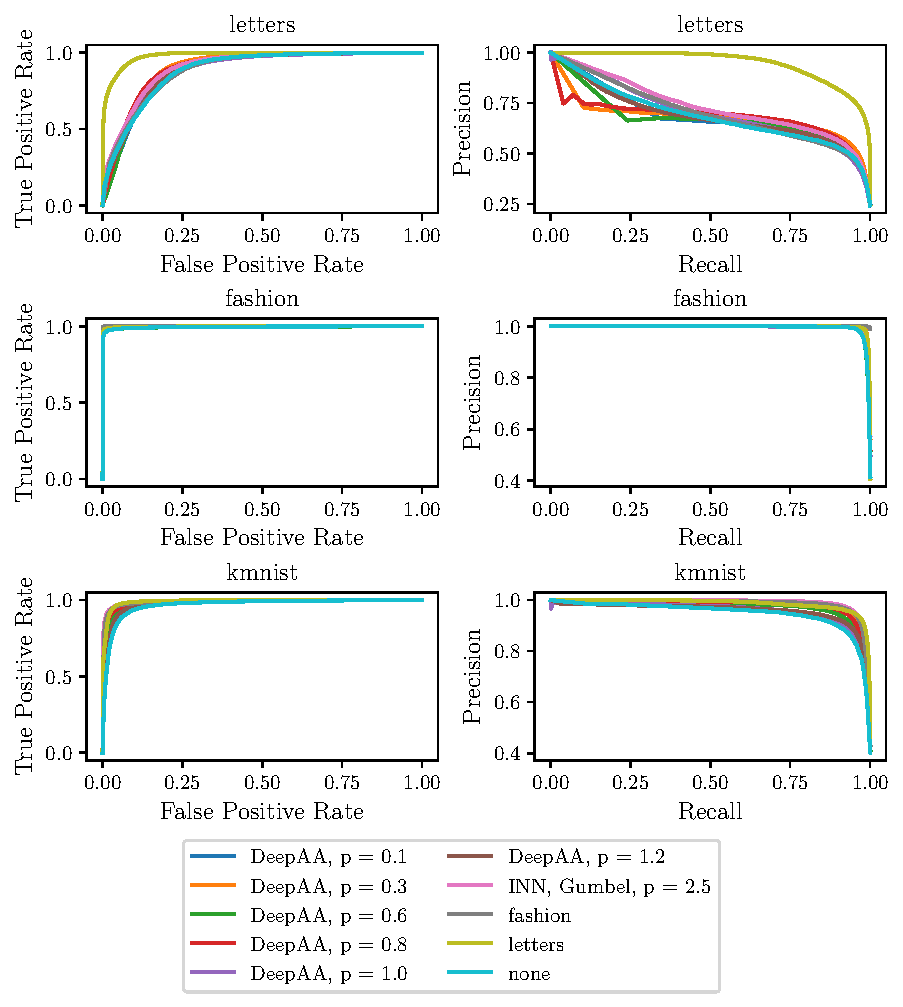
\includegraphics{figures/samples/emnist_class_curve.pdf}
    \caption{ROC curves (\textbf{left}) and precision-recall curve (\textbf{right}) for
    classifiers trained on different sources of outliers tested on different
    sources of outliers.}%
    \label{fig:emnist_stat_class}
\end{figure}

\begin{table}[htpb]
	\centering
        \caption{Area under the ROC curve (AUC) and average precision (AP) of
        discriminators trained on different outlier sources tested on different
        outlier datasets.}%
	\label{tab:emnist_disc}
	\begin{tabular}{lrrrrrr}
\toprule
{outliers} & \multicolumn{2}{c}{letters} & \multicolumn{2}{c}{fashion} & \multicolumn{2}{c}{kmnist} \\
{metric} & {AUC} & {AP} & {AUC} & {AP} & {AUC} & {AP} \\
\midrule
DeepAA, p = 0.1 & 0.64 & 0.33 & 0.88 & 0.77 & 0.67 & 0.47 \\
DeepAA, p = 0.3 & 0.57 & 0.27 & 0.52 & 0.37 & 0.46 & 0.34 \\
DeepAA, p = 0.5 & 0.48 & 0.22 & 0.38 & 0.31 & 0.42 & 0.33 \\
DeepAA, p = 0.6 & 0.47 & 0.22 & 0.39 & 0.32 & 0.37 & 0.31 \\
DeepAA, p = 0.8 & 0.43 & 0.20 & 0.48 & 0.35 & 0.39 & 0.32 \\
DeepAA, p = 1.2 & 0.45 & 0.21 & 0.74 & 0.51 & 0.63 & 0.42 \\
INN, Gumbel, p = 2.5 & 0.68 & 0.35 & 0.45 & 0.34 & 0.47 & 0.35 \\
INN, Normal, p = 1.5 & 0.58 & 0.27 & 0.12 & 0.25 & 0.38 & 0.32 \\
INN, Normal, p = 2.0 & 0.65 & 0.32 & 0.20 & 0.27 & 0.48 & 0.35 \\
INN, Normal, p = 2.5 & 0.69 & 0.39 & 0.80 & 0.61 & 0.72 & 0.50 \\
INN, Normal, p = 3.0 & 0.52 & 0.24 & 0.42 & 0.33 & 0.15 & 0.25 \\
fashion & 0.73 & 0.44 & \bfseries 1.00 & \bfseries 1.00 & \bfseries 0.97 & \bfseries 0.95 \\
letters & \bfseries 0.81 & \bfseries 0.56 & 0.50 & 0.36 & 0.48 & 0.35 \\
\bottomrule
\end{tabular}

\end{table}

\begin{table}[htpb]
	\centering
        \caption{Area under the ROC curve (AUC), average precision (AP) and
        test set classification accuracy (ACC) of classifiers trained on
        different outlier sources tested on different outlier datasets.}%
	\label{tab:emnist_class}
	\begin{tabular}{lrrrrrrrrr}
\toprule
{outliers} & \multicolumn{3}{c}{letters} & \multicolumn{3}{c}{fashion} & \multicolumn{3}{c}{kmnist} \\
{metric} & {AUC} & {AP} & {ACC} & {AUC} & {AP} & {ACC} & {AUC} & {AP} & {ACC} \\
\midrule
DeepAA, p = 0.1 & 0.89 & 0.64 & 1.00 & 1.00 & 1.00 & 1.00 & 0.99 & 0.98 & 1.00 \\
DeepAA, p = 0.3 & 0.90 & 0.66 & \bfseries 1.00 & 1.00 & 1.00 & \bfseries 1.00 & 0.99 & 0.99 & \bfseries 1.00 \\
DeepAA, p = 0.6 & 0.89 & 0.63 & 1.00 & 1.00 & 1.00 & 1.00 & 0.98 & 0.97 & 1.00 \\
DeepAA, p = 0.8 & 0.90 & 0.68 & 1.00 & 1.00 & 1.00 & 1.00 & 0.98 & 0.98 & 1.00 \\
DeepAA, p = 1.0 & 0.89 & 0.70 & 0.99 & 1.00 & 1.00 & 0.99 & 0.97 & 0.96 & 0.99 \\
DeepAA, p = 1.2 & 0.89 & 0.68 & 1.00 & 1.00 & 1.00 & 1.00 & 0.98 & 0.96 & 1.00 \\
INN, Gumbel, p = 2.5 & 0.90 & 0.72 & 1.00 & 1.00 & 1.00 & 1.00 & \bfseries 0.99 & \bfseries 0.99 & 1.00 \\
fashion & 0.89 & 0.67 & 1.00 & \bfseries 1.00 & \bfseries 1.00 & 1.00 & 0.99 & 0.99 & 1.00 \\
letters & \bfseries 0.98 & \bfseries 0.95 & 1.00 & 1.00 & 1.00 & 1.00 & 0.99 & 0.99 & 1.00 \\
none & 0.89 & 0.68 & 0.99 & 1.00 & 1.00 & 0.99 & 0.97 & 0.95 & 0.99 \\
\bottomrule
\end{tabular}

\end{table}

\begin{figure}[htpb]
    \centering
    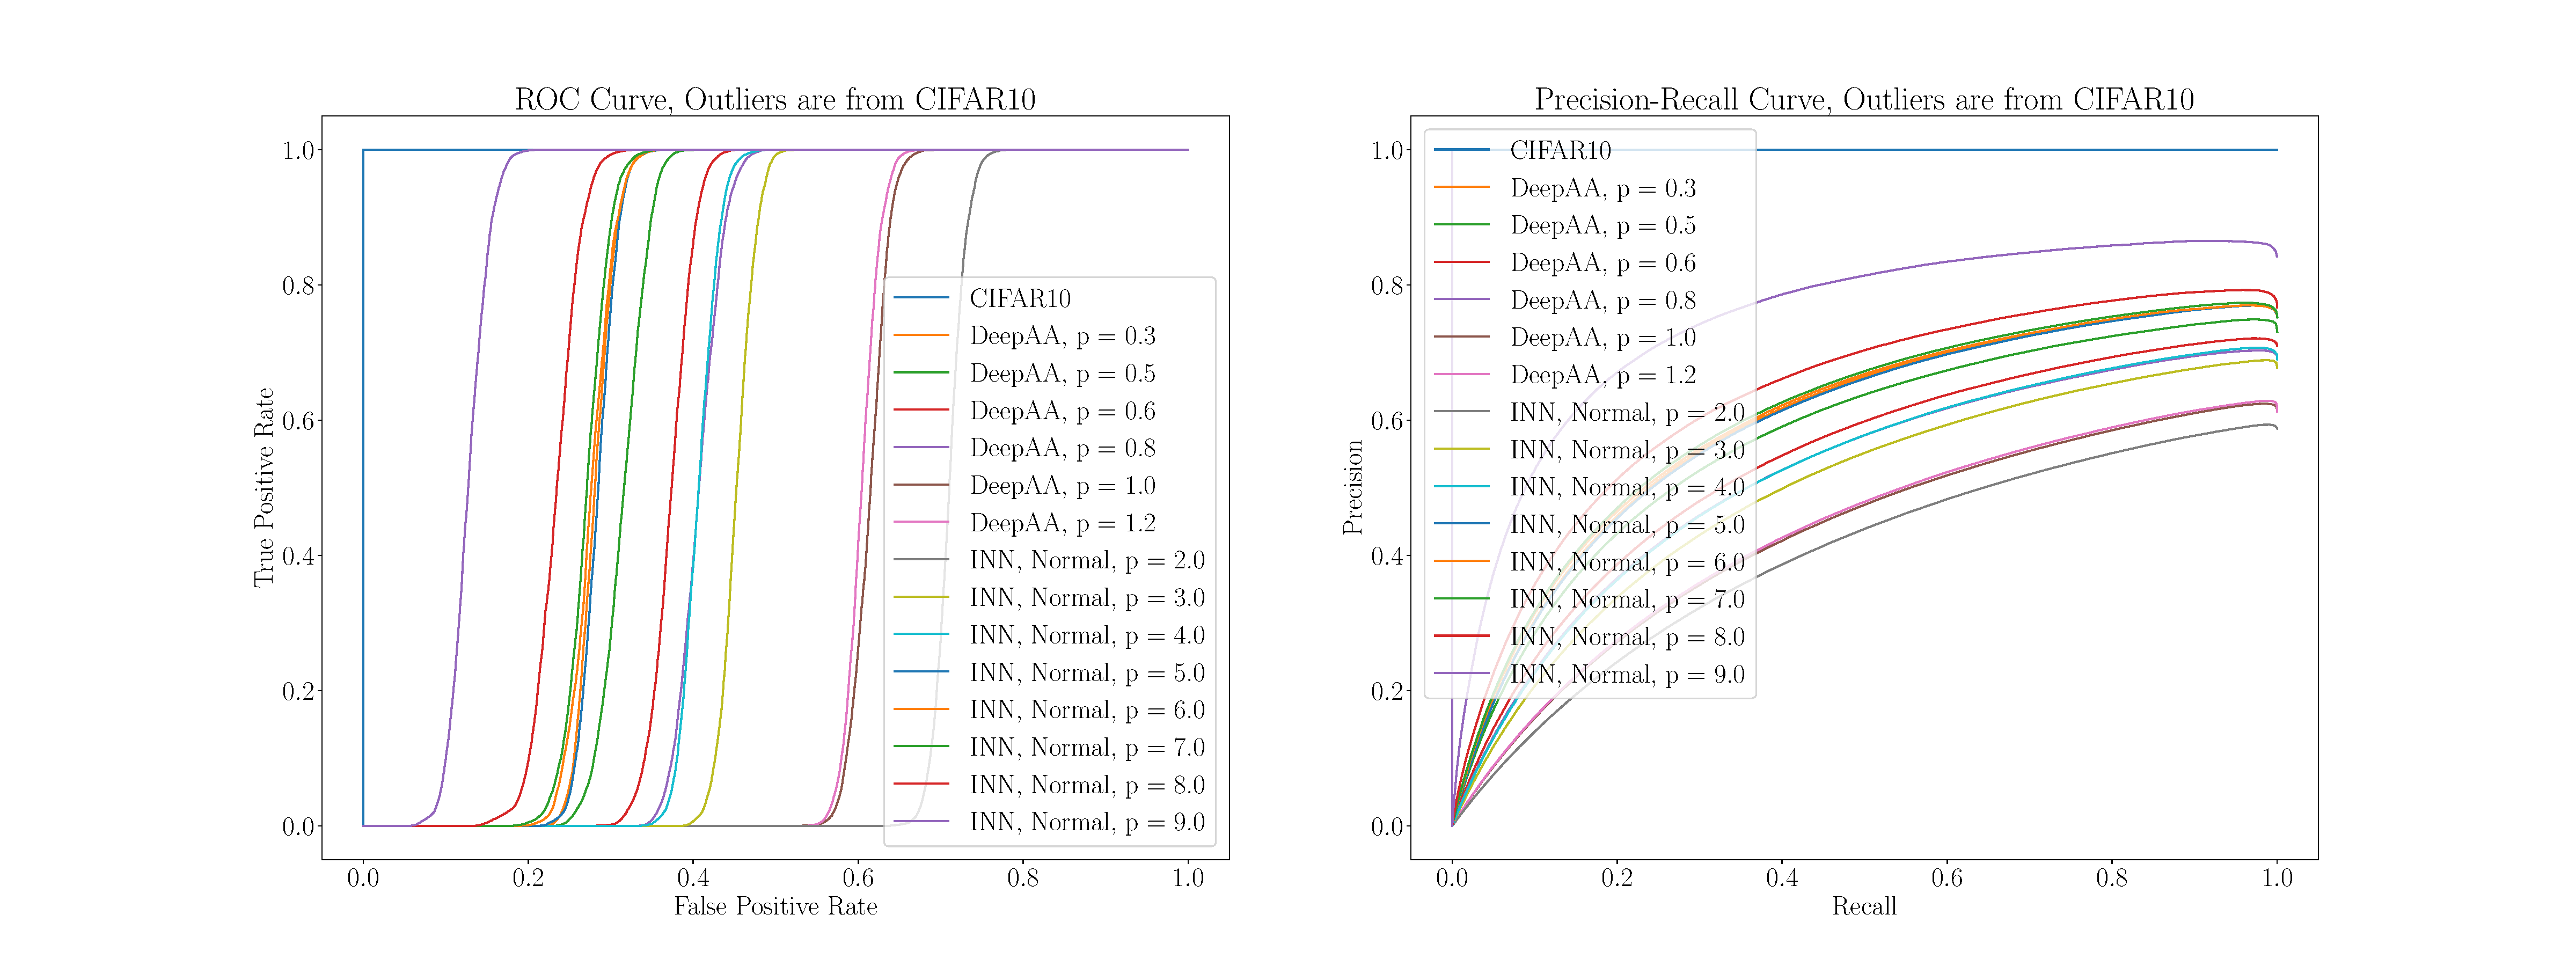
\includegraphics{figures/samples/ferg_CIFAR10_curve_disc.pdf}
    \caption{ROC curve (\textbf{left}) and precision-recall curve (\textbf{right}) for
        discriminators trained on different sources of outliers tested on
        different sources of outliers.}% 
    \label{fig:ferg_stat_disc}
\end{figure}

\begin{table}[htpb]
	\centering
        \caption{Area under the ROC curve (AUC) and average precision (AP) of
        discriminators trained on different outlier sources tested on different
        outlier datasets.}%
	\label{tab:ferg_disc}
	\begin{tabular}{lrr}
\toprule
{outliers} & \multicolumn{2}{c}{CIFAR10} \\
{metric} & {AUC} & {AP} \\
\midrule
CIFAR10 & \bfseries 1.00 & \bfseries 1.00 \\
DeepAA, p = 0.3 & 0.72 & 0.60 \\
DeepAA, p = 0.5 & 0.68 & 0.57 \\
DeepAA, p = 0.6 & 0.63 & 0.54 \\
DeepAA, p = 0.8 & 0.59 & 0.52 \\
DeepAA, p = 1.0 & 0.39 & 0.43 \\
DeepAA, p = 1.2 & 0.40 & 0.43 \\
INN, Normal, p = 2.0 & 0.29 & 0.40 \\
INN, Normal, p = 3.0 & 0.55 & 0.49 \\
INN, Normal, p = 4.0 & 0.59 & 0.52 \\
INN, Normal, p = 5.0 & 0.72 & 0.59 \\
INN, Normal, p = 6.0 & 0.72 & 0.60 \\
INN, Normal, p = 7.0 & 0.73 & 0.60 \\
INN, Normal, p = 8.0 & 0.77 & 0.63 \\
INN, Normal, p = 9.0 & 0.87 & 0.75 \\
\bottomrule
\end{tabular}

\end{table}

\begin{figure}[htpb]
    \centering
    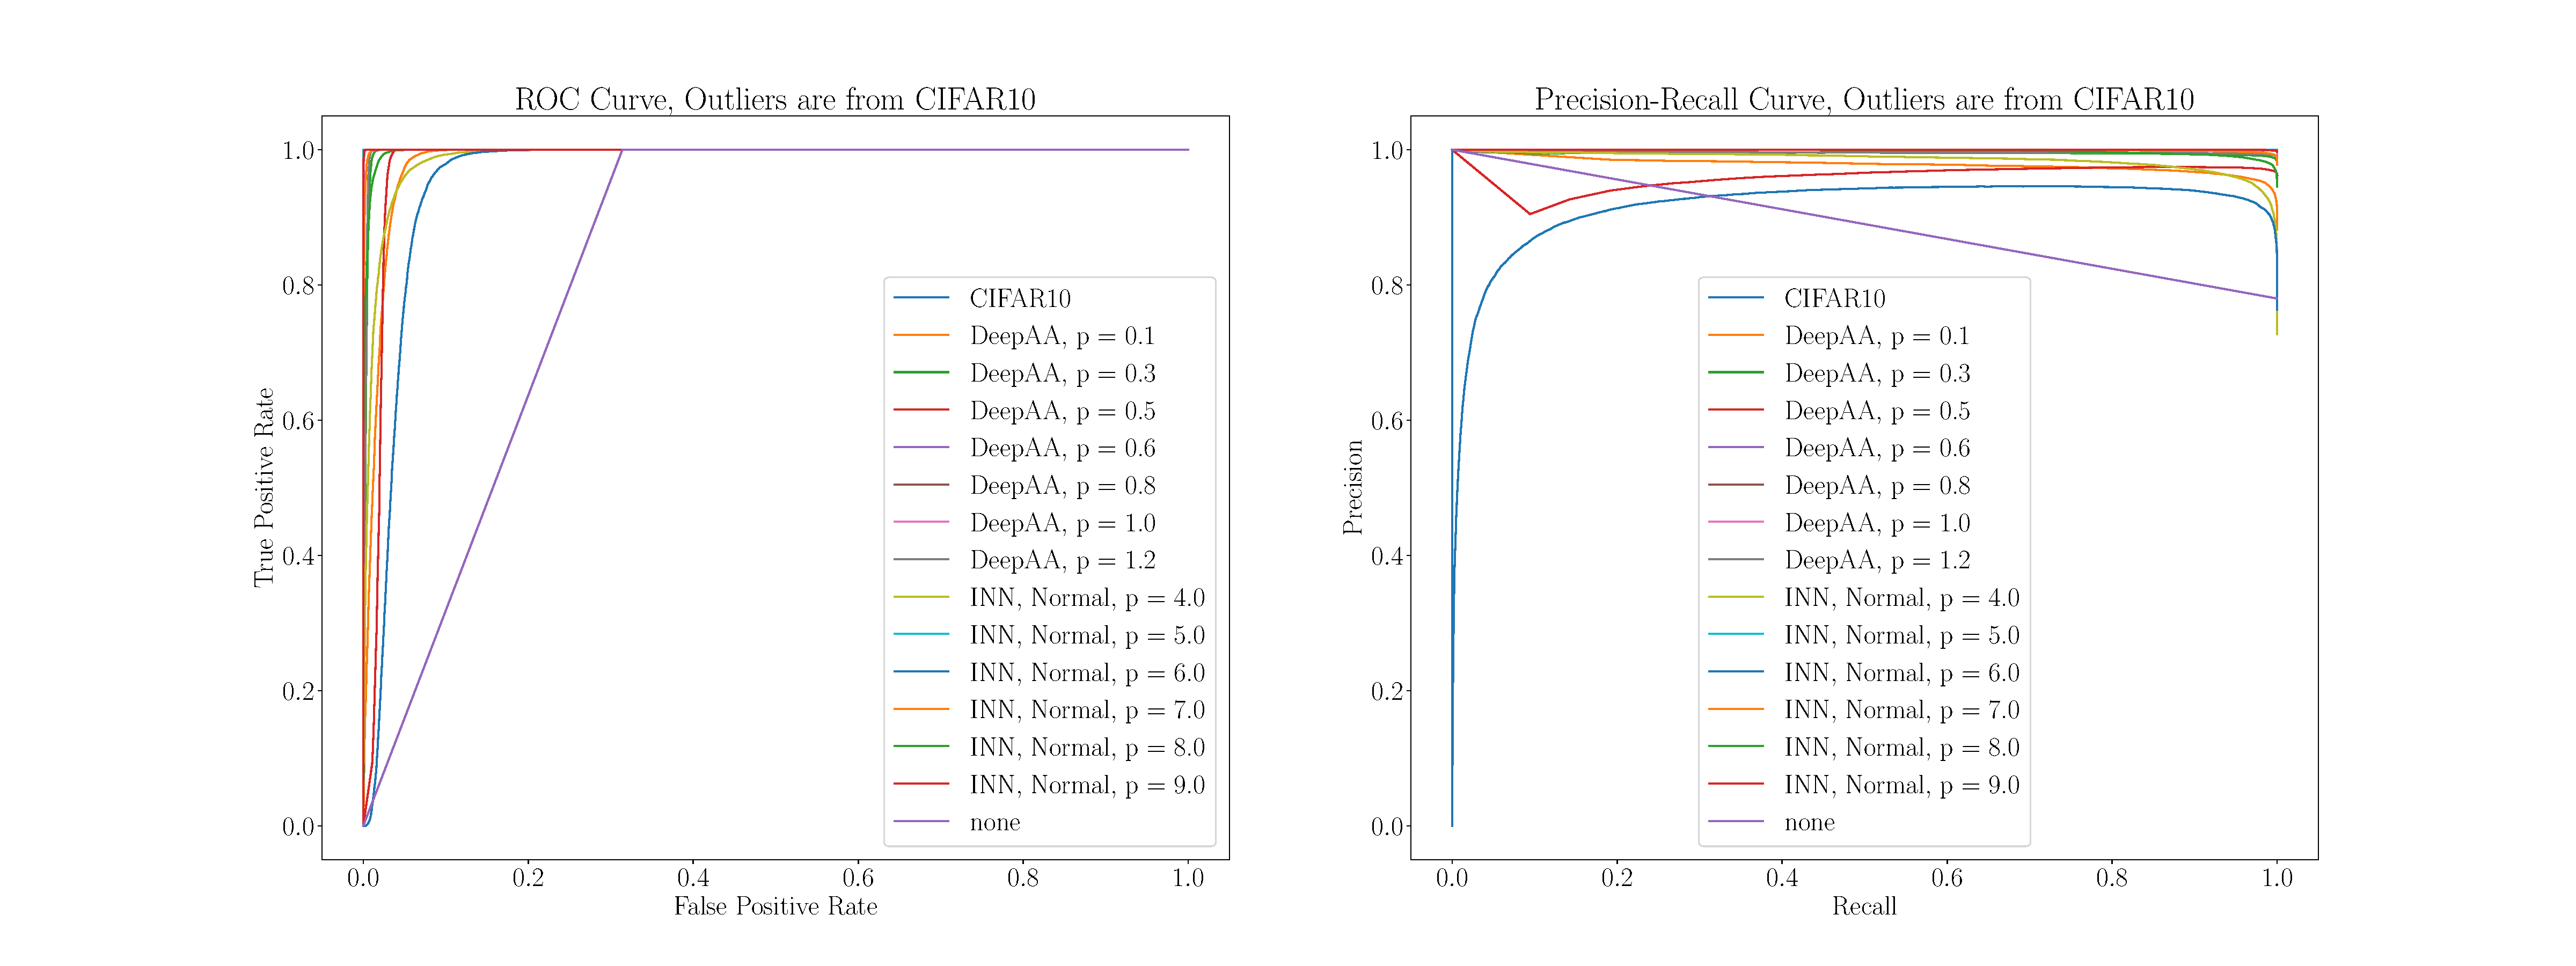
\includegraphics{figures/samples/ferg_CIFAR10_curve_class.pdf}
    \caption{ROC curve (\textbf{left}) and precision-recall curve (\textbf{right}) for
        classifiers trained on different sources of outliers tested on
        different sources of outliers.}% 
    \label{fig:ferg_stat_class}
\end{figure}

\begin{table}[htpb]
	\centering
        \caption{Area under the ROC curve (AUC), average precision (AP) and
        test set classification accuracy (ACC) of classifiers trained on
        different outlier sources tested on different outlier datasets.}%
	\label{tab:ferg_class}
	\begin{tabular}{lrrr}
\toprule
{outliers} & \multicolumn{3}{c}{CIFAR10} \\
{metric} & {AUC} & {AP} & {ACC} \\
\midrule
CIFAR10 & \bfseries 1.00 & \bfseries 1.00 & \bfseries 1.00 \\
DeepAA, p = 0.1 & 0.98 & 0.98 & \bfseries 1.00 \\
DeepAA, p = 0.3 & 1.00 & 0.99 & \bfseries 1.00 \\
DeepAA, p = 0.5 & 0.98 & 0.96 & \bfseries 1.00 \\
DeepAA, p = 0.6 & 1.00 & 1.00 & \bfseries 1.00 \\
DeepAA, p = 0.8 & 1.00 & 1.00 & \bfseries 1.00 \\
DeepAA, p = 1.0 & 1.00 & 1.00 & \bfseries 1.00 \\
DeepAA, p = 1.2 & 1.00 & 1.00 & \bfseries 1.00 \\
INN, Normal, p = 4.0 & 0.99 & 0.99 & \bfseries 1.00 \\
INN, Normal, p = 5.0 & 1.00 & 1.00 & \bfseries 1.00 \\
INN, Normal, p = 6.0 & 0.96 & 0.92 & \bfseries 1.00 \\
INN, Normal, p = 7.0 & 1.00 & 1.00 & \bfseries 1.00 \\
INN, Normal, p = 8.0 & 1.00 & 1.00 & \bfseries 1.00 \\
INN, Normal, p = 9.0 & 1.00 & 1.00 & \bfseries 1.00 \\
none & 0.84 & 0.78 & \bfseries 1.00 \\
\bottomrule
\end{tabular}

\end{table}
